\section{Current}
Current is the force that moves charge through a circuit. Current can be defined as an amount of charge moved over a time interval. This can be expressed as the following relation:
\begin{align}
i(t)=\dfrac{dq(t)}{dt} \Leftrightarrow q(t)=\int i(t)\ dt,
\label{I=dq/dt}
\end{align}
where $i(t)$ is the current (in ampere, $A$), to a given time $t$ (in seconds, $s$), and $q(t)$ is the function for charge at a given time $t$. $q(t)$ is measured in Coulomb $(C)$.
\\
There exists two types of current: alternating current (AC) and direct current (DC). Per definition, DC current is a constant flow of current, while AC alternates (see figure \ref{fig:ACDC}). 
\begin{figure}[H] 
\begin{tikzpicture}
\begin{axis}[ticks=none,
axis lines =center,
xlabel={t},
ylabel={i(t)},
    height=7cm, width=9cm,
    xmin=0, xmax=10, ymin=-2, ymax=2]
\addplot [
    domain=0:10, 
    samples=100, 
    color=red,
]
{1};
\addlegendentry{$DC$}
\addplot [
    domain=0:10, 
    samples=100, 
    color=blue,
    ]
    {sin(\x r)};
\addlegendentry{$AC$}
\end{axis}
\end{tikzpicture}
\caption{Current for AC and DC versus time}
\label{fig:ACDC}
\end{figure}
\noindent
A sinusoidal AC current can be described with the function: 
\begin{align}
i(t, f, A, \theta) =& A\cdot \sin{(2\pi ft + \theta)} \nonumber
\\
=& A \cdot \sin{(\omega t + \theta)} \label{eq:omega}
\end{align}
where $\omega = 2\pi f$, $t$ is time (in seconds, $s$), $f$ is frequency, which is cycles per second, (in Hertz, $Hz$), $A$ is amplitude (a scalar, unit-less), and $\theta$ is the phase-shift (in seconds, $s$).
For ease of understanding, $\omega$ is sometimes used for notation instead of $2\pi f$. $\omega$ is also called the angular frequency of the signal.
This function can be plotted as such:
\begin{figure}[H]
	\centering
	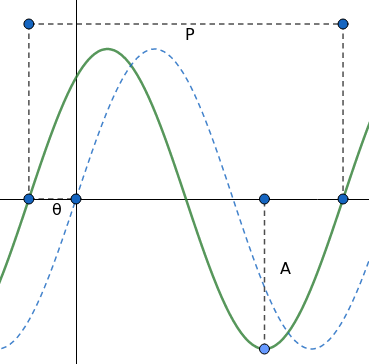
\includegraphics[scale=0.7]{fig/img/AC.png}
	\caption{An AC current, shown in green. The current has been phase-shifted by $\theta$. The current has amplitude $A$, and period $P=f^{-1}$. The dotted blue line shows the same current with $\text{phase-shift} =0$}
\end{figure}


\section{Voltage}
Voltage ($v$), also called electric potential difference, is the change in potential energy a charge undergoes, when it passes through two given points in a circuit. This is expressed in the following equation:
\begin{align}
	v=\dfrac{dU(q)}{dq},
\end{align}
\\
where $U(q)$ (in joules, $J$) is the function for potential energy, given a charge $q$.
\section{Resistor}
When a resistor, which is a passive element, is added to the circuit, it creates a resistance. Resistance makes it more difficult for the current to pass through the element. Resistance is defined as the proportional constant between current and voltage. The mathematical relation of this is given by:
\begin{align} 
\label{Ohm}
v(t)=R\cdot i(t),\ R\geq0,
\end{align}
where $R$ is resistance (in Ohm, $\Omega$). Furthermore, the power can be expressed as: \cite[p. 25]{bcircuit} 
\begin{align} 
\label{power}
p(t)=v(t)\cdot i(t)
\end{align}
By inserting this on equation \ref{Ohm} the following expression is found:
\begin{align}
p(t)=Ri(t)\cdot i(t) \\
p(t)=R \cdot i^2(t) \\
p(t)=R \cdot \left(\dfrac{v(t)}{R} \right)^2 \\
p(t)=\dfrac{v^2(t)}{R} \label{resistor:power}
\end{align}
The power is measuring the effect (in watts, $w$) This is defined as the amount of work done per time. 
\section{Capacitor}
A capacitor is a passive element of a circuit. A capacitor consists of two similar sized plates. When a voltage is applied to the circuit, the capacitor gets charged. The capacitance is the amount of energy a capacitor can store, when it is fully charged. The capacitor gets charged, when a positive charge is transferred from one plate to another through the circuit.
\\
The capacitance is given by the following equation:
\begin{align*}
C=\dfrac{\epsilon_{0}A}{d},
\end{align*}
where $C$ is the capacitance (in farad, $F$) and $\epsilon_{0}$ is the permittivity of free space, which is equal to $8.85 \cdot 10^{-12}                                                 \frac{F}{m}$. $A$ is the surface area of the plates (in square meters, $m^{2}$), and $d$ is the distance between the two plates (in meters, $m$).
\\
The charge of a capacitor across a voltage ($V$) and capacitance of ($C$) is equal to:
\begin{align}
\label{QCV}
q_C(t) = Cv_C(t)	
\end{align}
From \eqref{I=dq/dt}, current is defined as:
\begin{align*}
	i(t) = \frac{dq(t)}{dt}
\end{align*}
The current across a capacitor is then:
\begin{align*}
	i_C(t) = \frac{d}{dt}(Cv_C(t))
\end{align*}
For a capacitor with a constant capacitance, the current can be written as:
\begin{align}
	i_C(t) = C\frac{dv_C(t)}{dt}\label{iC}
\end{align}


\section{Time constant ($\tau$)}
A constant that shows up when looking at RC circuits, is the time constant $\tau = R \cdot C$, where $R$ is the resistance of the resistor, $C$ is the capacitance of the capacitor, and $\tau$ is time (in seconds, $s$).